% !TEX root = ../termpaper.tex
% first example sections
% @author Thomas Lehmann
%

\section{Simulation}
Im folgenden Kapitel werden die Simulationsergebnisse der hochselektiven Filterbank analysiert.

\subsection{Simulation der Teilbandausgänge}
Zunächst werden die Ausgänge der einzelnen Teilbänder simuliert. Hierzu werden die neun Ausgänge einzeln über den Frequenzbereich geplottet.\par
Abbildung \ref{fig:Teilband0} zeigt den Ausgang des ersten Teilbandes. Hier ist zu sehen, dass der Durchlassbereich bei den Frequenzen von $\frac{F_s}{4}$ bis $\frac{F_s}{2}$ liegt und somit gewünschte Hochpassverhalten zeigt.\par
\begin{figure}[h!]
	\centering	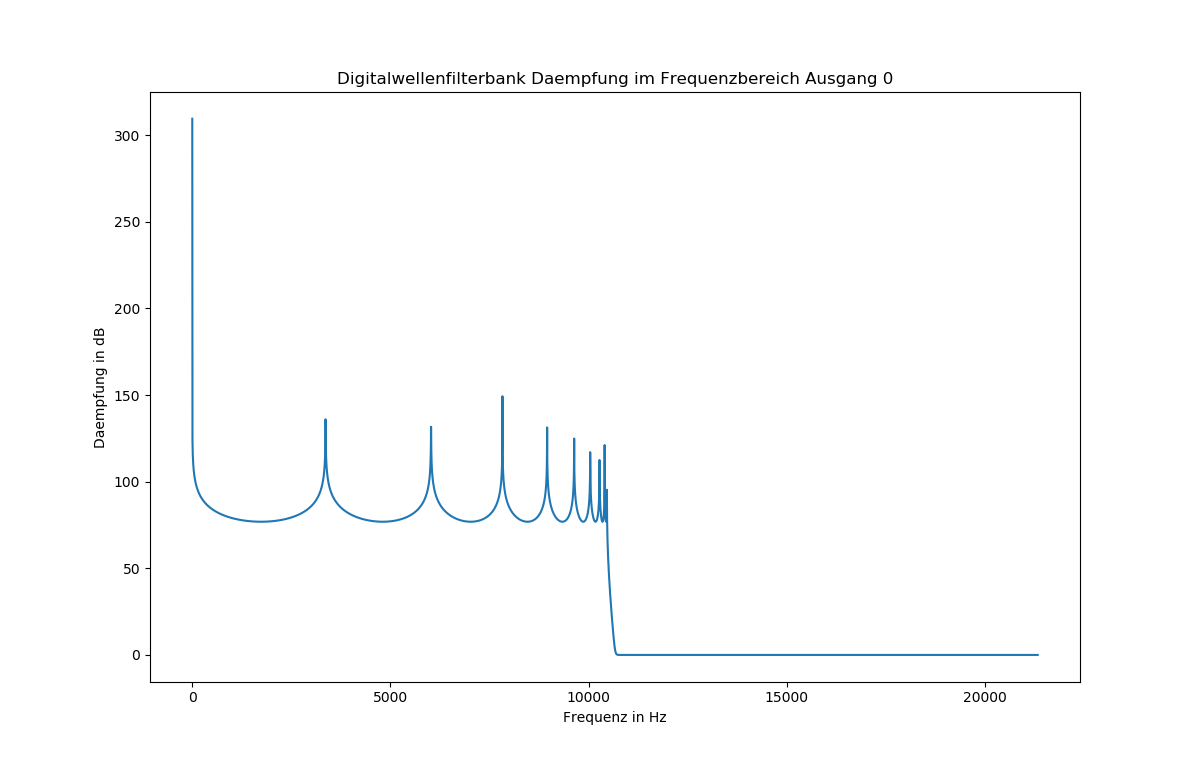
\includegraphics[width=14cm]{img/bank_freq_0.png}
	\caption{Ausgang des ersten Teilbandes}
	\label{fig:Teilband0}
\end{figure}
Ein weiteres exemplarisches Teilband zeigt Abbildung \ref{fig:Teilband5} mit dem sechsten Teilband. Hierbei ist der erkennen, dass das Teilband den erwarteten Frequenzbereich von 375 bis 750\,Hz durchlässt.\par
\begin{figure}[h!]
	\centering	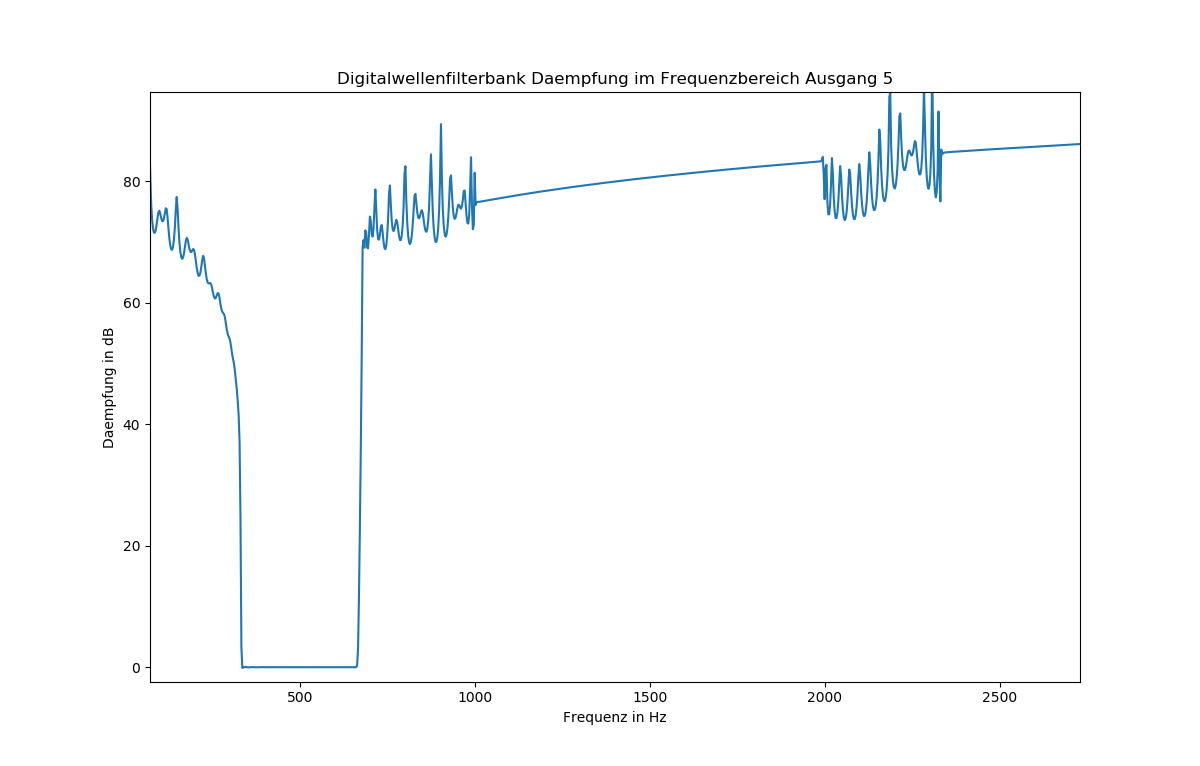
\includegraphics[width=14cm]{img/bank_freq_5_close.png}
	\caption{Ausgang des sechsten Teilbandes}
	\label{fig:Teilband5}
\end{figure}
Die restlichen Teilbänder zeigen ebenfalls den erwarteten Durchlassbereich.

\subsection{Simulation der Signallaufzeiten}
Nachfolgend werden die Signallaufzeiten der einzelnen Teilbänder simuliert und zusammen in einem Plot dargestellt (siehe Abbildung \ref{fig:TeilbandLaufzeitenohne}). Zu erkennen ist, dass ein Ausgleich der einzelnen Signallaufzeiten nötig ist.\par
\begin{figure}[h!]
	\centering	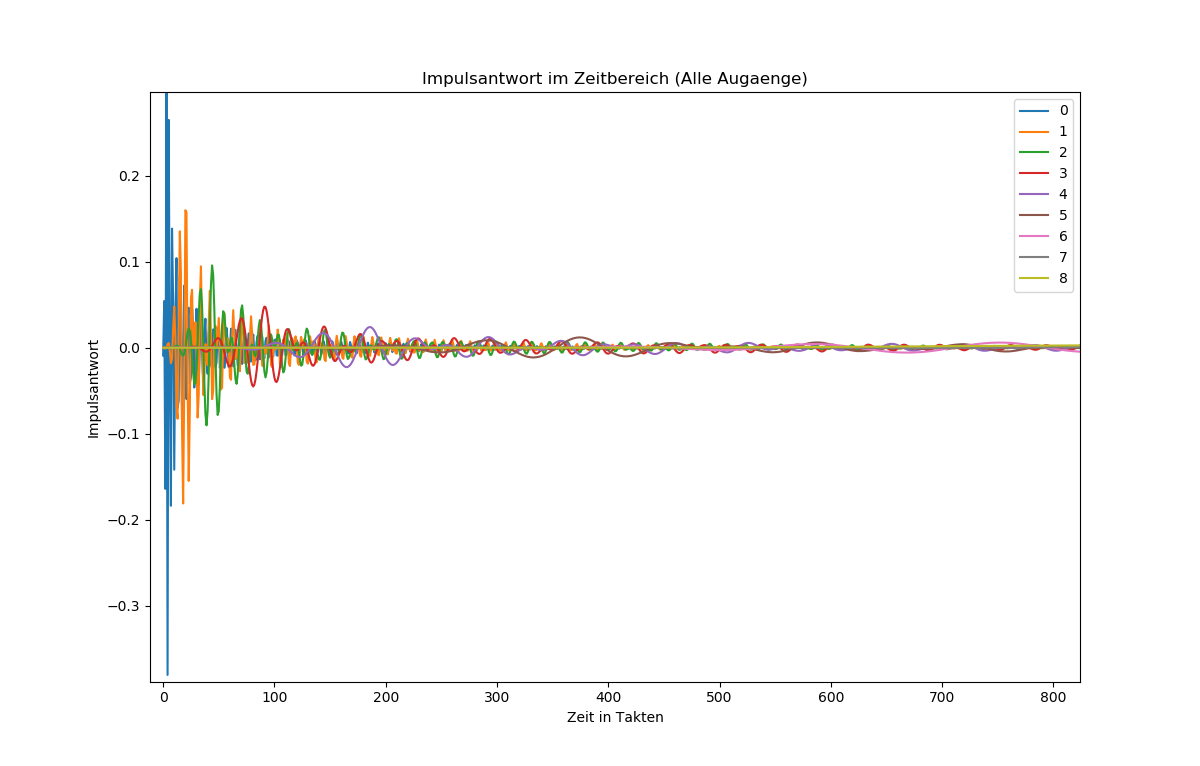
\includegraphics[width=15cm]{img/bank_zeit_alle_keinAusgleich.png}
	\caption{Signallaufzeiten der Teilfilterbänder ohne Ausgleich}
	\label{fig:TeilbandLaufzeitenohne}
\end{figure}
Die einzelnen laufzeitbereinigten Impulsantworten der Teilbänder zeigen das Maximum ungefähr nach 1500 Takten (siehe Abbildung \ref{fig:TeilbandLaufzeiten}). Somit kann das ursprüngliche Signal am Ausgang wieder zusammengesetzt werden.
\begin{figure}[h!]
	\centering	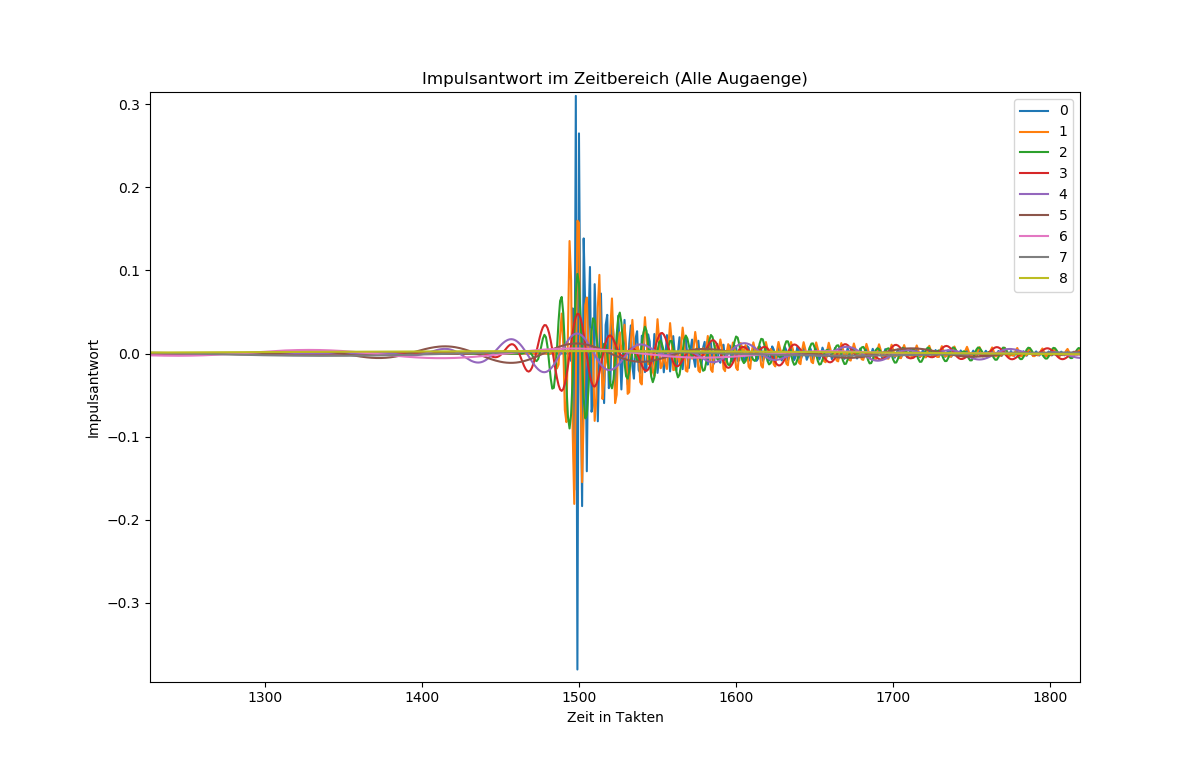
\includegraphics[width=15cm]{img/bank_zeit_alle.png}
	\caption{Signallaufzeiten der Teilfilterbänder}
	\label{fig:TeilbandLaufzeiten}
\end{figure}

\subsection{Simulation des Oktav-Filterbank-Ausgangs}
Abschließend wird die gesamte Oktav-Filterbank simuliert. In Abbildung \ref{fig:OktavLaufzeit} sieht man die Signallaufzeit der Filterbank. Zu erkennen ist bei $t$ = 0 der Impuls am Eingang. Nach den erwarteten 1500 Takten wird der Impuls am Ausgang ausgegeben.\par
\begin{figure}[h!]
	\centering	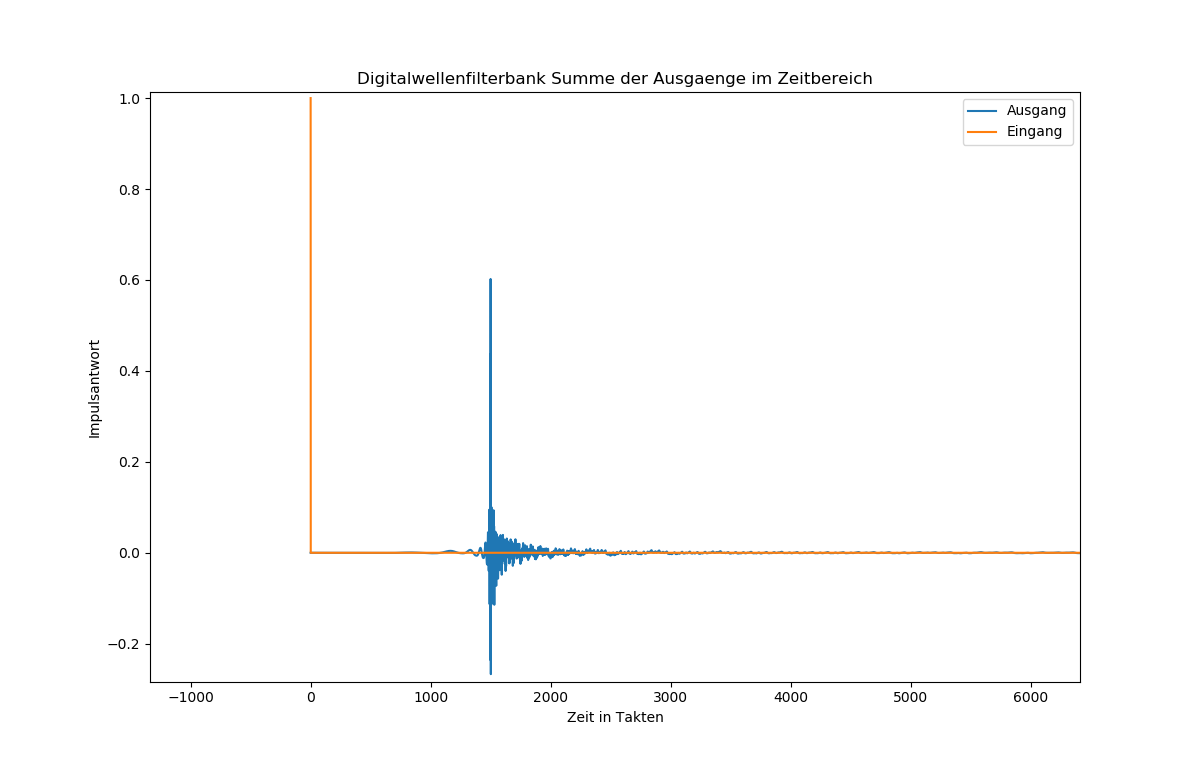
\includegraphics[width=14cm]{img/bank_zeit_summe.png}
	\caption{Signallaufzeit der Summe der Oktav-Filterbank}
	\label{fig:OktavLaufzeit}
\end{figure}
Abbildung \ref{fig:AusgangDeampfungohneAusgleich} zeigt die Dämpfung der Filterbank ohne Laufzeitausgleich. In Abbildung \ref{fig:AusgangDeampfung} hingegen ist die Dämpfung der Filterbank mit Laufzeitausgleich zu sehen. Wie zu erkennen ist, verbessert sich die Dämpfung an den Übergängen der einzelnen Teilbänder durch den Laufzeitausgleich. Die Abweichungen an den Übergängen der einzelnen Teilbänder sind durch die unterschiedlichen Phasengänge bedingt. Hierdurch ist die Verzögerung nicht bei allen Frequenzen optimal. Ein weiterer Punkt sind numerische Rundungsfehler, wodurch das Ergebnis ebenfalls leicht verfälscht wird und die Übergänge der Teilbandfilter nicht optimal sind. Die Impulsantworten der niederfrequenten Teilbänder sind zum Ende der Simulation noch nicht vollständig Ausgeschwungen (siehe Abbildung \ref{fig:Ausschwingen}). 
\begin{figure}[h!]
	\centering	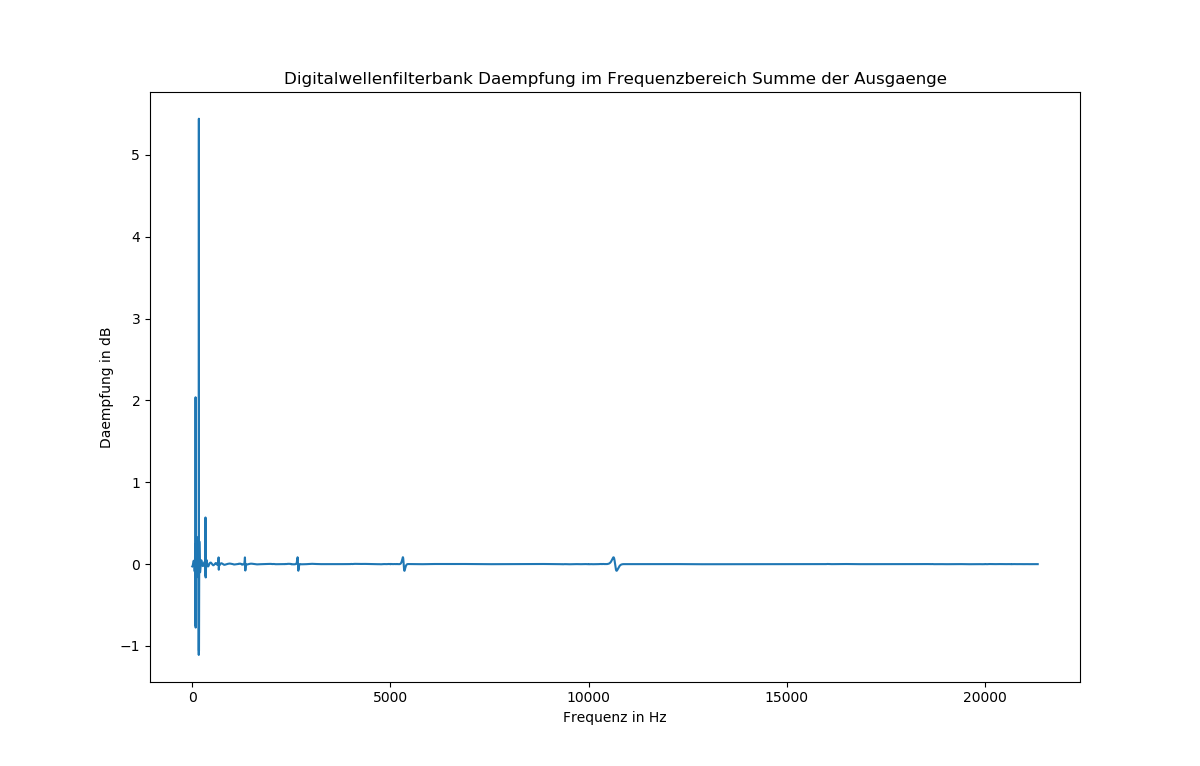
\includegraphics[width=14cm]{img/bank_freq_summe_keinAusgleich.png}
	\caption{Dämpfung der Oktav-Filterbank ohne Laufzeitausgleich}
	\label{fig:AusgangDeampfungohneAusgleich}
\end{figure}
\begin{figure}[h!]
	\centering	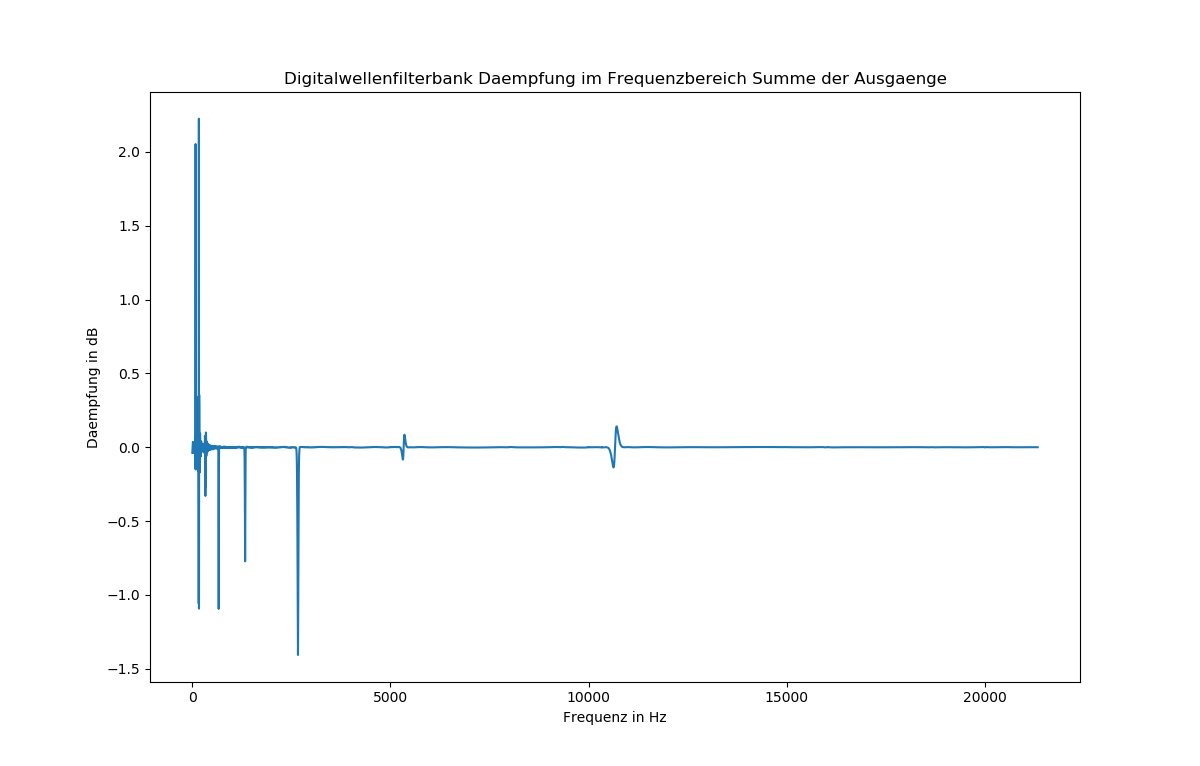
\includegraphics[width=14cm]{img/bank_freq_summe.png}
	\caption{Dämpfung der Oktav-Filterbank mit Laufzeitausgleich}
	\label{fig:AusgangDeampfung}
\end{figure}
\begin{figure}[h!]
	\centering	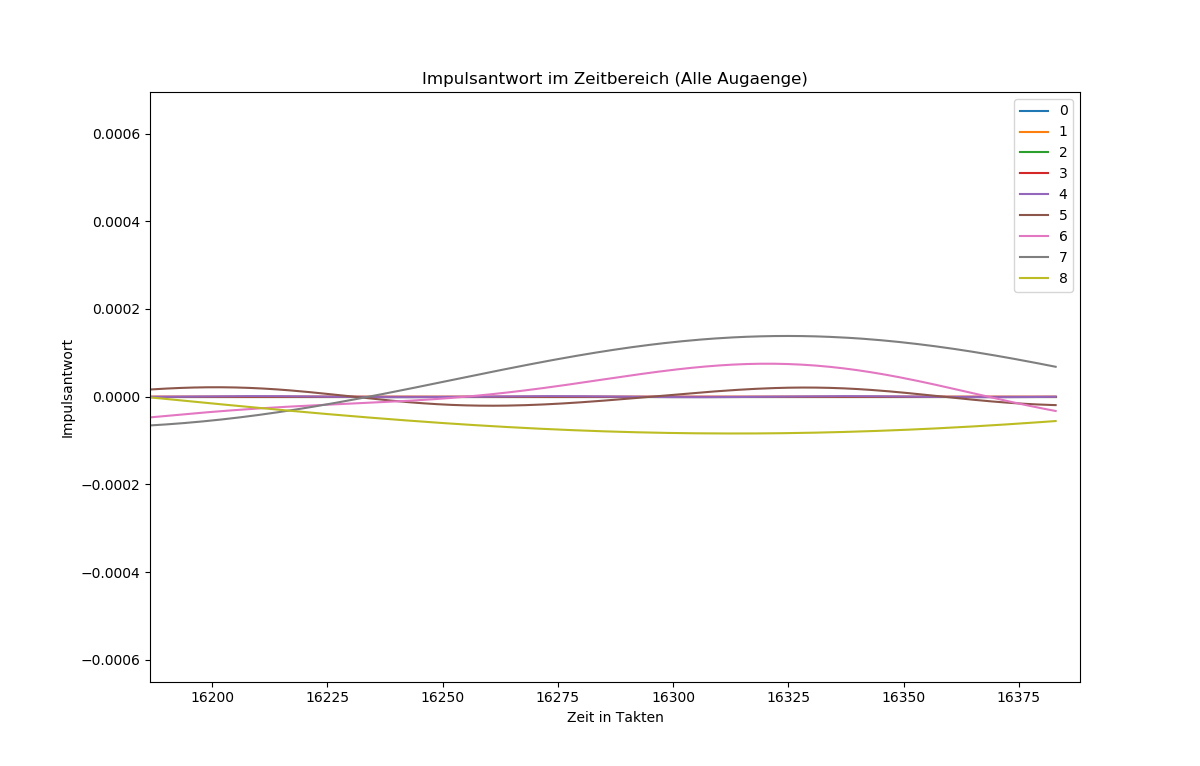
\includegraphics[width=14cm]{img/bank_zeit_alle_ausschwingen.png}
	\caption{Ausschwingen der niederfrequenten Teilbänder}
	\label{fig:Ausschwingen}
\end{figure}